\documentclass[12pt,a4paper]{article}
\usepackage[utf8]{inputenc}
\usepackage[T1]{fontenc}
\usepackage{amsmath}
\usepackage{amsfonts}
\usepackage{amssymb}
\usepackage{graphicx}
\usepackage[indonesian]{babel}
\usepackage[left=2.00cm, right=2.00cm, top=2.00cm, bottom=2.00cm]{geometry}
\usepackage{float} 

\title{Tugas 14 - Pengolahan Sinyal Digital\\
	Disain Filter Digital FIR}

% remove spacing around date:
\usepackage{titling}
\predate{}
\postdate{}
\date{}

\begin{document}
	\maketitle
	\date{}
	\begin{enumerate}
		\item Dalam metode window dalam desain filter FIR lowpass, kita sudah tunjukkan bahwa lebar transisi dari filter yang dihasilkan tergantung pada lebar main lobe dari transformasi Fourier dari windownya. Untuk tujuan dari permasalahan ini, kita definisikan main lobe sebagai interval simetris antara frekuensi negatif dan positif pertama di mana $ W(e^{j\omega}) = 0 $. Perhatikan tiga window berikut:
		
		\begin{figure}[H]
			\centering
			
\includegraphics[width=0.7\linewidth]{img/img01}
		\end{figure}
		
		(Jika $ \alpha = \beta = 0.5 $ maka ini adalah Hanning window. Jika $ \alpha = 0.54 $ dan $ \beta = 0.46 $ maka ini adalah Hamming window.)\\
		
		
		Tentukan transformasi Fourier dari tiap window di atas. Tentukan juga lebar dari main lobe dari tiap window tersebut, asumsikan $ N >> 1 $\\
		
		\pagebreak
		\textbf{Jawaban:}
		
		\textbf{Rectangular window:}
		
		\begin{figure}[H]
			\centering
			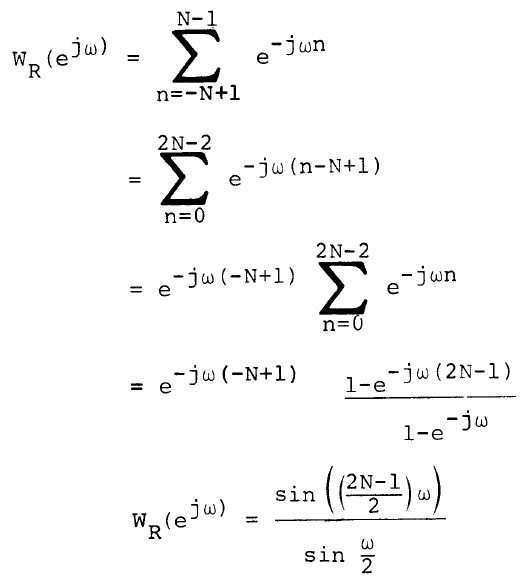
\includegraphics[width=0.6\linewidth]{img/img02}
		\end{figure}
		
		Sehingga lebar main lobe adalah $ \frac{4 \pi}{2N - 1} $ yang mana untuk $ N >> 1 $ kurang lebih lebar main lobe adalah $ \frac{2 \pi}{N} $
		
		\pagebreak
		\textbf{Bartlett window:}
		
		Diketahui: 
		
		\begin{figure}[H]
			\centering
			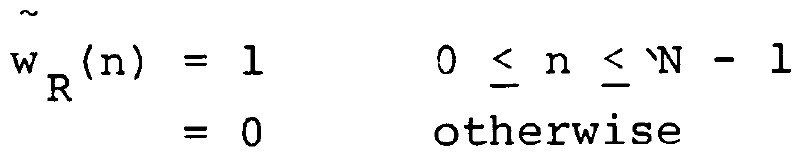
\includegraphics[width=0.4\linewidth]{img/img03}
		\end{figure}
		
		Maka 
		
		\begin{figure}[H]
			\centering
			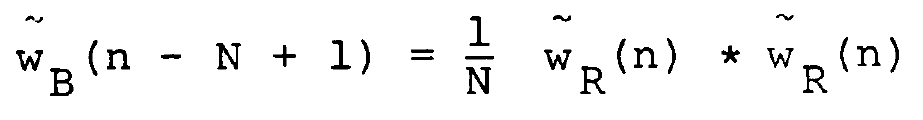
\includegraphics[width=0.4\linewidth]{img/img04}
		\end{figure}
		
		Berdasarkan persamaan 7.76 di Referensi utama (dengan $ N = M + 1 $)
		
		\begin{figure}[H]
			\centering
			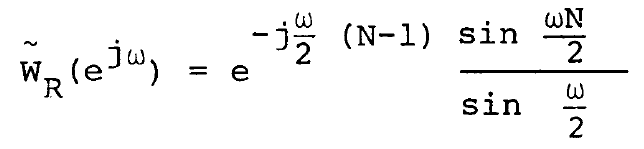
\includegraphics[width=0.4\linewidth]{img/img05}
		\end{figure}
		
		Sehingga
		
		\begin{figure}[H]
			\centering
			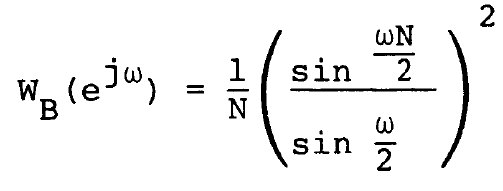
\includegraphics[width=0.4\linewidth]{img/img06}
		\end{figure}
		
		Pada kasus seperti ini, lebar dari main lobe adalah $ 4\pi / N $ yang mana ini adalah dua kalinya dari rectangular window.
		
		\pagebreak
		\textbf{Raised cosine window}
		
		\begin{figure}[H]
			\centering
			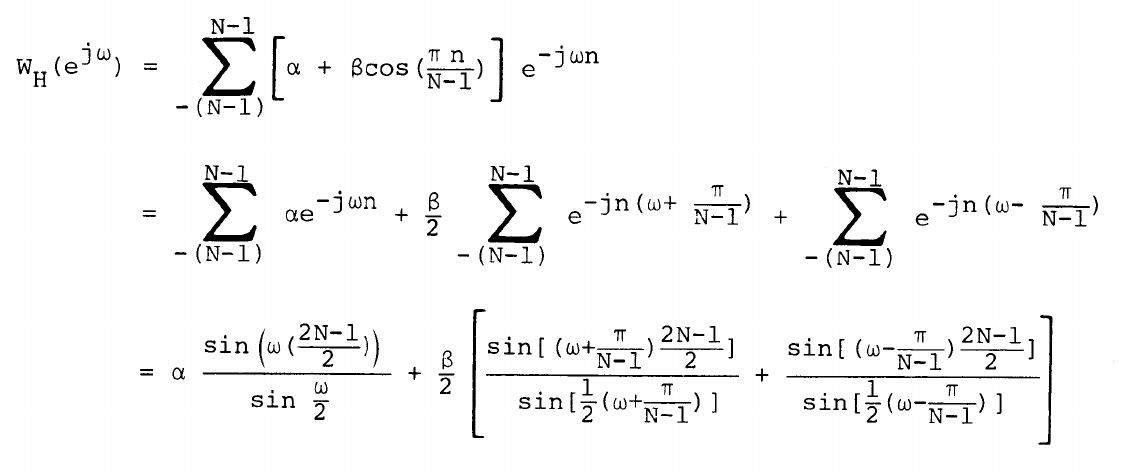
\includegraphics[width=0.8\linewidth]{img/img07}
		\end{figure}
		
		Asumsikan $ N >> 1 $, maka bentuk di atas dapat ditulis kembali menjadi
		
		\begin{figure}[H]
			\centering
			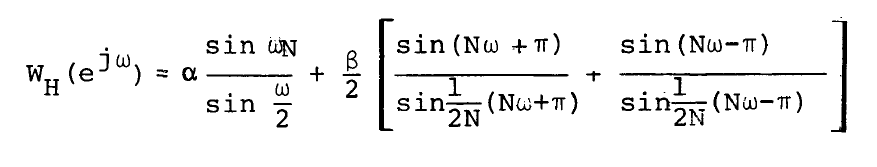
\includegraphics[width=0.8\linewidth]{img/img08}
		\end{figure}
		
		Bentuk di atas merupakan superposisi dari 3 bentuk seperti pada gambar di bawah
		
		\begin{figure}[H]
			\centering
			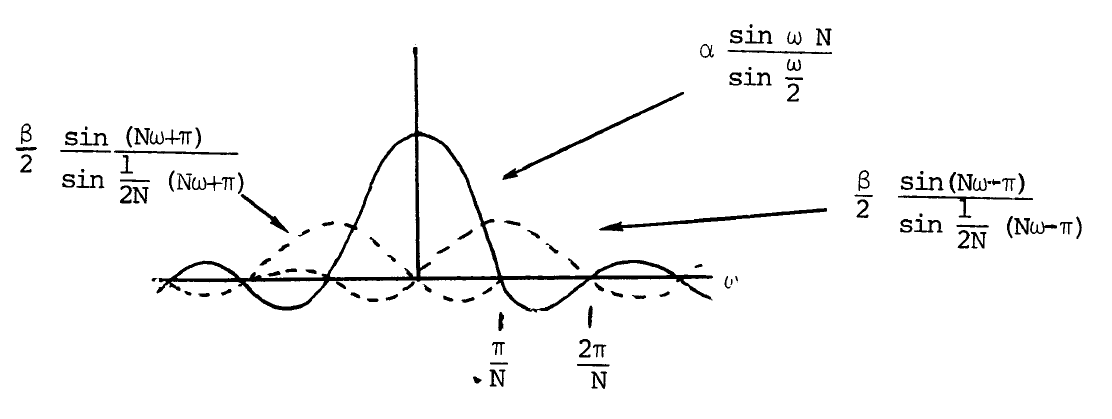
\includegraphics[width=\linewidth]{img/img09}
		\end{figure}
		
		Berdasarkan gambar di atas, kita dapatkan bahwa nilai pertama dari $ \omega $ dimana superposisinya akan menjadi nol adalah $ \omega = \pm 2\pi / N $. Akibatnya lebar main lobe-nya adalah $ 4\pi / N $
	\end{enumerate}
\end{document}